\documentclass[conference]{IEEEtran}

\usepackage{amsmath,amssymb}
\usepackage{graphicx}
\usepackage{booktabs}
\usepackage{multirow}
\usepackage{cite}
\usepackage{url}
\usepackage{microtype}
\usepackage{balance}

\title{Adaptive Observation-Efficient Power Transformer Fault Diagnosis from Partial DGA Histories Using Explainable Lightweight Machine Learning}

\author{\IEEEauthorblockN{Taufikur Rahman Fuad}
\IEEEauthorblockA{Department of Electrical and Electronic Engineering\\
Islamic University of Technology (IUT)\\
Gazipur, Bangladesh}}

\begin{document}
\maketitle

\begin{abstract}
Most machine-learning studies for dissolved gas analysis (DGA) evaluate fault classification only after the complete monitoring record is available. For condition-based maintenance, the more useful question is how much history is actually required for a reliable decision, whether that requirement varies by case, and how the feature representation should change as evidence accumulates. This paper extends an observation-efficient transformer-diagnosis framework on a public benchmark containing 3,000 multivariate DGA histories, each with 420 twelve-hour measurements of H$_2$, CO, C$_2$H$_4$, and C$_2$H$_2$. The supplied 2,100/900 train-test split is preserved and all shorter-horizon features are computed from leakage-safe prefixes. In the canonical experiment, an 82-feature temporal logistic-regression model reaches 0.8971 macro-F1 at 75\% history and 0.9026 at 100\%, retaining 99.39\% of its endpoint performance. A direct paired difference-of-differences test confirms a horizon--representation interaction: $(T_{75}-S_{75})-(T_{100}-S_{100})=0.0761$ with 95\% CI $[0.0278,0.1263]$. A dense 10--100\% study shows that the temporal advantage is concentrated mainly in the intermediate-history regime rather than being universal. A stopping policy selected exclusively from training out-of-fold predictions ($\tau=0.95$, persistence $K=3$) achieves 0.8865 test macro-F1, retains 98.29\% of its endpoint reference, and requires only 37.8\% history on average; the median stopping horizon is 20\%, and 93.6\% of cases stop before the endpoint. Fixed-horizon class-conditional conformal prediction reaches 90.56\% empirical coverage at a nominal 90\% target at 75\% history. Redundancy analysis further shows that the nominal 82-feature representation has numerical rank 70, and a compact 36-feature statistical-plus-endpoint representation captures much of the 75\%-history benefit. Finally, stress testing exposes a severe sensitivity to independently injected high-frequency multiplicative noise; removing algebraic redundancy and applying a training-selected causal moving average raises macro-F1 from 0.2476 to 0.6250 at 2\% noise while preserving clean performance near 0.896. The results support an adaptive stop/continue/defer architecture in which observation duration, feature representation, uncertainty, and robustness are treated as coupled engineering design variables.
\end{abstract}

\begin{IEEEkeywords}
power transformer, dissolved gas analysis, fault diagnosis, time series, adaptive stopping, explainable AI, conformal prediction, robustness, condition monitoring
\end{IEEEkeywords}

\section{Introduction}
Consider a transformer for which 315 DGA measurements have already been collected. At the 12-hour sampling interval of the benchmark used here, those measurements represent 157.5 nominal sampling-days. A conventional endpoint evaluation waits for another 105 measurements before issuing its final diagnosis. The first practical question is simple: \emph{does that final quarter of the record materially improve the diagnosis, or is the model already close to its endpoint performance?} A second question is more demanding: \emph{should every transformer be forced to wait for the same fraction of history, or can sufficiently clear cases stop earlier while ambiguous cases continue under observation?}

These questions matter because power transformers are high-value assets whose failures can disrupt transmission and distribution, create safety risks, and impose substantial repair and outage costs. Dissolved gas analysis is one of the principal techniques used to monitor mineral-oil-immersed transformers. IEEE Std C57.104-2019 and IEC 60599:2022 relate dissolved-gas concentrations and their evolution to electrical and thermal fault processes and emphasize engineering interpretation rather than a single automated threshold \cite{ieeeC57104,iec60599}. The physical basis is well established: electrical discharges and thermal degradation generate characteristic gases in transformer oil, allowing incipient conditions to be investigated without dismantling the unit \cite{rogers1978,cheng2018survey,ali2023review,nanfak2024review}.

Machine learning has substantially expanded DGA interpretation. Support-vector machines, tree ensembles, clustering, evidence-fusion methods, and other intelligent models have produced strong fault-classification results \cite{zhang2019khsvm,shang2019hmsvm,liu2020dbscan,hechifa2024ensemble,lv2024lightgbm,zhang2022copula}. Recent reviews increasingly argue that the field should move beyond headline accuracy toward sound validation, robustness, interpretability, and practical transferability \cite{bouzar2026robustness}. That motivates a different experiment from the usual model leaderboard: instead of asking only which classifier performs best after the complete record is available, we ask \emph{how diagnostic quality evolves as the observation window grows, when additional temporal complexity is useful, and when enough evidence has accumulated to stop observing}.

The public Power Transformers FDD and RUL benchmark makes these questions testable. It contains 3,000 labeled multivariate histories, each with 420 measurements of H$_2$, CO, C$_2$H$_4$, and C$_2$H$_2$, sampled every 12 hours. The four classes are normal mode, partial discharge, low-energy discharge, and low-temperature overheating \cite{katserDataset}. The supplied split contains 2,100 training and 900 test cases and is strongly imbalanced: normal operation accounts for more than 81\% of the held-out cases. Work on the same benchmark lineage has already shown that engineered time-series features and classical machine learning can achieve high endpoint performance \cite{katser2022}. We therefore do not propose another large neural architecture. Instead, we make observation duration a controlled experimental variable and deliberately keep the predictive model lightweight.

The present paper retains the canonical partial-history study and adds four extensions that materially change the engineering interpretation:
\begin{itemize}
    \item We preserve the leakage-safe 25/50/75/100\% experiment and strengthen its central result with a direct paired difference-of-differences test. The horizon--representation interaction is positive by 0.0761 macro-F1 with 95\% CI $[0.0278,0.1263]$.
    \item We densify the observation grid to 10, 15, 20, \ldots, 100\% and show that temporal descriptors are not universally superior: they are most useful in an intermediate partial-history regime, while the 25\% and endpoint regions favor or match compact statistical summaries.
    \item We replace a globally fixed operating point with a training-selected adaptive policy. On the held-out test set, the selected policy stops at 37.8\% history on average while retaining 98.29\% of the corresponding endpoint macro-F1.
    \item We add fixed-horizon class-conditional conformal uncertainty, horizon-specific SHAP analysis, redundancy-aware feature-family ablation, and controlled robustness tests. The robustness study deliberately reports a severe noise failure of the original representation and a targeted mitigation based on nonredundant features and causal smoothing.
\end{itemize}

The central claim is therefore stronger, but also more specific, than in a conventional endpoint-classification paper. Observation duration, feature representation, stopping policy, uncertainty, and robustness are coupled engineering design variables. A useful condition-monitoring system should decide not only \emph{what} fault class is most plausible, but also \emph{when} enough evidence exists to issue that diagnosis and \emph{when} continued monitoring or expert review remains necessary.

\section{Observation-Efficient Diagnosis Framework}
\subsection{Partial-History Formulation}
Let the $i$th transformer history be $\mathbf{X}_i\in\mathbb{R}^{T\times G}$, where $T=420$ time points and $G=4$ gas channels. Its label $y_i$ belongs to the four diagnostic classes. For observation fraction $h$, only the prefix
\begin{equation}
\mathbf{X}_i^{(h)}=\mathbf{X}_i[1:T_h,:],\qquad T_h=\mathrm{round}(hT)
\label{eq:prefix}
\end{equation}
is exposed before feature extraction. The canonical experiment uses $h\in\{0.25,0.50,0.75,1.00\}$. The dense extension uses $h\in\{0.10,0.15,\ldots,1.00\}$. A 50\%-history slope, last value, late-period mean, or maximum change therefore terminates at sample 210; no information from samples 211--420 is allowed. This prefix-first rule is essential because computing temporal descriptors from the complete sequence and then evaluating them at a shorter horizon would leak future information.

We evaluate a performance curve $M(h)$ rather than a single endpoint score. Macro-F1 is the primary metric because the class distribution is highly imbalanced. A fixed observation-efficient operating point is a horizon $h<1$ for which $M(h)$ is close to $M(1)$. The adaptive extension instead permits each case $i$ to stop at its own horizon $h_i$, provided a training-selected persistence rule is satisfied.

\subsection{Feature Representations}
The canonical study compares three representations. The \emph{snapshot} baseline contains only the final observed value of each gas at the current horizon (4 features). The \emph{statistical} representation uses seven descriptive statistics per gas---mean, standard deviation, minimum, maximum, median, 25th percentile, and 75th percentile---for 28 features. The \emph{full temporal} representation contains 82 columns: the statistical summaries plus first and last values, total change, linear slope, trend $R^2$, first-difference statistics, maximum absolute step change, early and late means, late-minus-early change, fraction of positive differences, and six pairwise gas correlations.

The refinement study audits algebraic dependence inside the 82-column representation. In particular, for a prefix of length $N$,
\begin{equation}
\Delta x=x_{\mathrm{last}}-x_{\mathrm{first}},\qquad
\overline{\Delta x}=\frac{\Delta x}{N-1},
\end{equation}
and the late-minus-early descriptor is exactly the difference between two already included segment means. The 82-column matrix therefore has numerical rank 70. A nonredundant \emph{Temporal-70} representation removes these exact dependencies while preserving the same broad feature families. We additionally isolate compact groups---endpoint levels, trend, local roughness, segment levels, and cross-gas correlations---to test which temporal information actually adds value beyond Statistical-28.

For the final robustness refinement, Statistical-28 is computed from the raw observed prefix, while the nonredundant temporal additions may be computed from a causal moving-average signal. For window $w$, the smoothed value at time $t$ uses only samples at or before $t$,
\begin{equation}
\tilde{x}_t=\frac{1}{\min(w,t)}\sum_{j=\max(1,t-w+1)}^{t}x_j,
\end{equation}
so the preprocessing does not introduce future leakage.

\subsection{Lightweight Classification and Adaptive Stopping}
For all principal experiments, standardized features feed multinomial logistic regression. Given class scores $p_k(\mathbf{x})$, the predicted class is
\begin{equation}
\hat{y}=\arg\max_k p_k(\mathbf{x}),
\end{equation}
and the native maximum score is
\begin{equation}
s(\mathbf{x})=\max_k p_k(\mathbf{x}).
\end{equation}
The canonical selective-diagnosis analysis compares $s(\mathbf{x})$ with a fixed threshold and treats low-score cases as deferred. These scores are used for ranking and abstention; no claim is made that the native logistic-regression score is perfectly calibrated.

The adaptive extension evaluates a sequence of dense horizons. A case stops at horizon $h_j$ only if two conditions hold for $K$ consecutive horizons: the predicted class is unchanged and the score is at least $\tau$. The policy parameters $(\tau,K)$ are selected exclusively from five-fold out-of-fold (OOF) predictions on the training set. Eligible policies must retain at least 97\% of endpoint OOF macro-F1 and maintain every class recall at or above 0.75. Among eligible policies, the one with the smallest mean OOF stopping horizon is selected. The held-out test partition is used once after this policy is fixed.

\begin{figure*}[t]
    \centering
    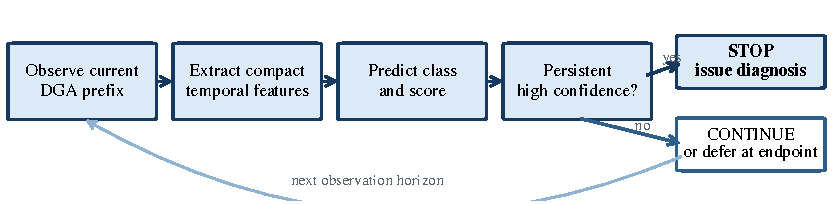
\includegraphics[width=0.97\textwidth]{figures/adaptive_pipeline.pdf}
    \caption{Adaptive observation-efficient diagnosis pipeline. Features are recomputed from the currently available prefix; a case stops only after persistent high-score evidence supports the same class. Otherwise monitoring continues, and unresolved endpoint cases can be deferred for engineering review.}
    \label{fig:pipeline}
\end{figure*}

\subsection{Conformal Decision Sets}
To complement score-based abstention, we use class-conditional split conformal prediction at fixed horizons \cite{angelopoulos2023conformal}. The 2,100-case training partition is split internally into a proper training subset and a calibration subset with stratification. For class $k$, calibration nonconformity is $1-p_k(\mathbf{x})$ evaluated on examples whose true label is $k$. A class-specific empirical quantile determines whether each label is included in the prediction set. We use nominal miscoverage $\alpha=0.10$. The fixed-horizon coverage and set-size results are the formal uncertainty analysis. Reusing these sets sequentially across horizons is reported only as exploratory because ordinary split-conformal guarantees do not automatically become anytime-valid under optional stopping.

\section{Dataset and Experimental Protocol}
\subsection{Dataset and Class Distribution}
The Power Transformers FDD and RUL dataset provides 3,000 labeled histories under a CC0 license \cite{katserDataset}. Each history contains 420 measurements at 12-hour intervals for H$_2$, CO, C$_2$H$_4$, and C$_2$H$_2$. The supplied split is preserved exactly: 2,100 training cases and 900 test cases. Table~\ref{tab:data} shows the class distribution.

\begin{table}[t]
\caption{Dataset class distribution.}
\label{tab:data}
\centering
\footnotesize
\begin{tabular}{lrr}
\toprule
Class & Train & Test \\
\midrule
Normal mode & 1705 & 731 \\
Partial discharge & 89 & 38 \\
Low-energy discharge & 113 & 49 \\
Low-temperature overheating & 193 & 82 \\
\midrule
Total & 2100 & 900 \\
\bottomrule
\end{tabular}
\end{table}

Because 731 of 900 test cases are normal, raw accuracy alone can hide poor minority-fault performance. We therefore report macro-F1, balanced accuracy, class-wise precision/recall/F1, and class-specific coverage in addition to overall accuracy.

\subsection{Canonical Model Selection}
The 900-case test partition is never used for model selection or hyperparameter tuning. On the 2,100 training cases, we use stratified five-fold cross-validation with shuffling and random seed 42. The primary selection metric is macro-F1. All models are implemented in scikit-learn \cite{pedregosa2011}.

The canonical experiment compares five lightweight model families on the complete 82-feature representation: logistic regression, RBF-kernel support-vector machine, random forest, Extra Trees, and histogram gradient boosting. Logistic regression is selected by training-CV macro-F1 and tuned over $C\in\{0.01,0.03,0.1,0.3,1,3,10,30,100\}$ and class-weight options \{balanced, none\}. The best canonical five-fold setting is $C=30$ with no class weighting, giving training-CV macro-F1 0.9151. That configuration is frozen across the canonical 25/50/75/100\% representation studies.

\subsection{Protocol Separation for the Extensions}
The later experiments are extensions of the canonical study rather than silent replacements for it. This distinction matters because the canonical paper archive was fitted under its original numerical solver configuration. The advanced dense-horizon, adaptive-stopping, conformal, SHAP-stability, and stress-test analyses keep $C=30$ and no class weighting but use a tighter logistic-regression tolerance of $10^{-6}$ to improve numerical convergence. The saved canonical predictions remain the source for the primary 75\%-versus-100\% formal interaction test.

The final redundancy/noise refinement separately reruns the original 18-combination $(C,\text{class weight})$ grid under the $10^{-6}$ tolerance. Training-only CV selects $C=100$ with balanced class weighting, with mean macro-F1 0.91587. The second-best configurations are extremely close, so this later winner is treated as a convergence-stable refinement rather than evidence that the original $C=30$ model was conceptually wrong. The refinement configuration is used only for the nonredundant feature and noise-mitigation study; it does not overwrite the canonical paper metrics.

\subsection{Metrics, Paired Resampling, and Interaction Test}
For class $k$, precision, recall, and F1 are denoted $P_k$, $R_k$, and $F1_k$. Macro-F1 is
\begin{equation}
F1_{\mathrm{macro}}=\frac{1}{4}\sum_{k=1}^{4}F1_k.
\label{eq:macrof1}
\end{equation}
Balanced accuracy is the mean class recall. Canonical point estimates receive nonparametric 95\% bootstrap confidence intervals from 5,000 test-set resamples. Paired method comparisons resample the same held-out transformer indices for both methods.

To test whether the temporal representation changes value with horizon, we use the paired difference-of-differences
\begin{equation}
D=\left(F1_{T,75}-F1_{S,75}\right)-\left(F1_{T,100}-F1_{S,100}\right),
\label{eq:interaction}
\end{equation}
where $T$ and $S$ denote Temporal-82 and Statistical-28. The 95\% interval is obtained from 5,000 paired bootstrap resamples of the same 900 test cases. Dense per-horizon intervals are descriptive pointwise intervals and are not adjusted for multiple comparisons; the pre-specified 75\%-to-100\% interaction is the primary inferential comparison.

\subsection{Controlled Robustness Tests}
The 75\%-history model is also tested under synthetic measurement imperfections without retraining: random missing timestamps, one contiguous gap, gradual single-gas multiplicative drift, and independent multiplicative Gaussian noise. Missing samples and gaps are linearly interpolated. Stress levels are 5/10/20\% for missingness, gaps, and drift and 2/5/10\% for Gaussian noise, with 20 Monte Carlo repeats. These tests are controlled stress experiments, not field validation and not assertions that the percentages correspond to a calibrated sensor-error distribution.

The final mitigation study selects a causal moving-average window from $w\in\{1,3,5,7,11\}$ using training OOF data only. Candidate windows must preserve at least 98\% of the unsmoothed clean OOF macro-F1. Among eligible candidates, the highest mean OOF score under 2\% and 5\% training-side Gaussian stress is chosen. Independent test perturbation seeds are then used for the final evaluation.

\section{Results}
\subsection{Canonical Benchmark and Endpoint Performance}
Table~\ref{tab:models} reports the canonical five-fold benchmark. Logistic regression obtains the highest training-CV macro-F1 (0.9094), so it is selected for tuning. Histogram gradient boosting happens to achieve the highest test macro-F1 in the untuned benchmark, but that held-out result is not used to change the selected model family.

\begin{table*}[t]
\caption{Canonical lightweight model benchmark on the full 82-feature history. Model selection uses five-fold training-CV macro-F1, not held-out test performance.}
\label{tab:models}
\centering
\footnotesize
\begin{tabular}{lcccc}
\toprule
Model & CV macro-F1 & Test accuracy (\%) & Test balanced accuracy & Test macro-F1 \\
\midrule
Logistic regression & $\mathbf{0.9094}\pm0.0169$ & 94.33 & \textbf{0.9408} & 0.8879 \\
RBF SVM & $0.8706\pm0.0101$ & 96.44 & 0.9078 & 0.9157 \\
Random forest & $0.8595\pm0.0336$ & 96.22 & 0.8925 & 0.9058 \\
Extra Trees & $0.8722\pm0.0261$ & 96.56 & 0.8865 & 0.9141 \\
Histogram gradient boosting & $0.8935\pm0.0199$ & \textbf{97.11} & 0.9283 & \textbf{0.9213} \\
\bottomrule
\end{tabular}
\end{table*}

After tuning, canonical logistic regression reaches five-fold training-CV macro-F1 0.9151. On the untouched 900-case test set it achieves 96.00\% accuracy, 0.9105 balanced accuracy, 0.9026 macro-F1, and 0.9608 weighted F1. The 95\% bootstrap interval for test macro-F1 is $[0.8664,0.9343]$. Normal operation reaches F1 0.9821, partial discharge 0.9189, low-energy discharge 0.8571, and low-temperature overheating 0.8523. The confusion matrix in Fig.~\ref{fig:cm} shows 864 correct predictions.

\begin{figure}[t]
    \centering
    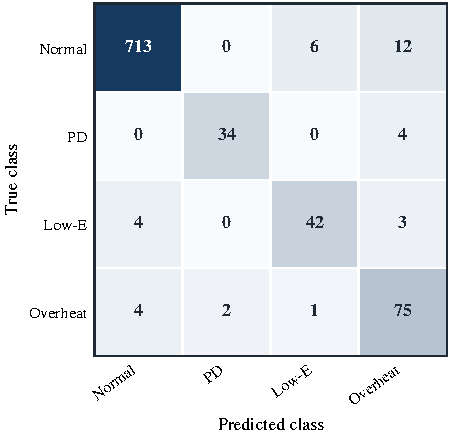
\includegraphics[width=0.96\columnwidth]{figures/confusion_matrix_final.pdf}
    \caption{Canonical confusion matrix for the tuned 82-feature logistic-regression model at 100\% history.}
    \label{fig:cm}
\end{figure}

\subsection{Canonical Partial-History Result and Formal Interaction}
At the complete history, the four-value snapshot reaches 0.9061 test macro-F1, Statistical-28 reaches 0.9232, and Temporal-82 reaches 0.9026. A full-history-only study would therefore conclude that additional temporal descriptors are unnecessary. The partial-history experiment shows why that conclusion is incomplete.

\begin{table*}[t]
\caption{Canonical horizon--representation results on the same 900 held-out cases. $\Delta$ is Temporal-82 minus Statistical-28 macro-F1.}
\label{tab:horizon}
\centering
\footnotesize
\begin{tabular}{cccccc}
\toprule
History & Nominal days & Statistical-28 & Temporal-82 & $\Delta$ & 95\% CI for $\Delta$ \\
\midrule
25\% & 52.5 & \textbf{0.7313} & 0.6752 & $-0.0561$ & $[-0.1078,-0.0046]$ \\
50\% & 105.0 & 0.7801 & \textbf{0.8108} & $+0.0307$ & $[-0.0148,0.0789]$ \\
75\% & 157.5 & 0.8417 & \textbf{0.8971} & $\mathbf{+0.0555}$ & $\mathbf{[0.0102,0.1013]}$ \\
100\% & 210.0 & \textbf{0.9232} & 0.9026 & $-0.0206$ & $[-0.0537,0.0109]$ \\
\bottomrule
\end{tabular}
\end{table*}

Within Temporal-82, 75\% history retains
\begin{equation}
\frac{0.8971}{0.9026}\times100\%=99.39\%
\end{equation}
of endpoint macro-F1 while using 105 fewer twelve-hour observations. The observed 100\%-minus-75\% difference is 0.0055 with paired 95\% CI $[-0.0271,0.0364]$. This interval is not an equivalence test; it shows that the measured endpoint gain is small and uncertain. Statistical-28 behaves differently, rising from 0.8417 at 75\% to 0.9232 at 100\%, a gain of 0.0815 with paired 95\% CI $[0.0422,0.1249]$.

The direct interaction test removes the ambiguity of comparing those intervals separately. At 75\%, the temporal-minus-statistical effect is $+0.05547$; at 100\%, it is $-0.02059$. Their paired difference is
\begin{equation}
D=0.07607,
\end{equation}
with 95\% CI $[0.02785,0.12631]$. The interval lies entirely above zero. The evidence therefore supports a genuine horizon--representation interaction between the pre-specified 75\% and 100\% points.

\subsection{Dense Horizons: Temporal Value Is Concentrated in the Middle}
Figure~\ref{fig:dense} extends the observation grid from four horizons to 19 horizons at 5\%-point spacing. The result is more informative than a claim that ``75\% is optimal.'' Temporal-82 is weaker than Statistical-28 at 25\% ($\Delta=-0.0517$, pointwise 95\% CI $[-0.1031,-0.0019]$), begins to gain at intermediate horizons, and shows its clearest positive region from approximately 55\% to 75\%. The observed temporal-minus-statistical macro-F1 differences are $+0.0521$ at 55\%, $+0.0636$ at 60\%, $+0.0492$ at 65\%, $+0.0567$ at 70\%, and $+0.0487$ at 75\%; the corresponding pointwise intervals exclude zero. At 80\% the interval crosses zero, and by the endpoint Statistical-28 again has the higher point estimate.

\begin{figure}[t]
    \centering
    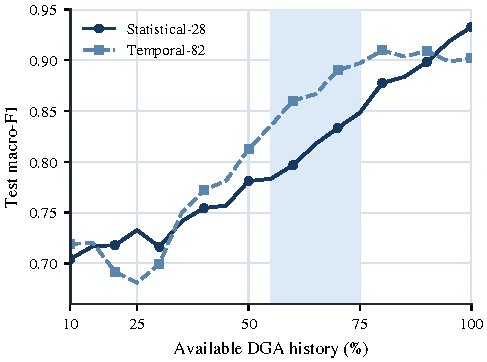
\includegraphics[width=\columnwidth]{figures/dense_horizon_representation.pdf}
    \caption{Dense held-out performance from 10\% to 100\% history under the convergence-stabilized extension. Temporal descriptors provide their clearest incremental value in an intermediate partial-history regime.}
    \label{fig:dense}
\end{figure}

This dense curve changes the interpretation in an important way. Temporal complexity is not automatically rewarded whenever the record is incomplete. At the shortest horizons, extra dynamic descriptors are unstable or uninformative; in the middle of the trajectory they add useful change information; near the endpoint the accumulated distributional summaries become highly competitive. Observation duration and representation should therefore be designed jointly rather than selected independently.

\subsection{Adaptive Stopping Replaces a Single Global Horizon}
The training OOF search selects $\tau=0.95$ and persistence $K=3$. On training OOF predictions, the policy retains 97.65\% of endpoint macro-F1 and keeps minimum class recall at 0.796, satisfying the predeclared constraints. On the untouched test set, the frozen policy obtains 95.56\% accuracy, 0.8947 balanced accuracy, and 0.8865 macro-F1, compared with a 0.9019 endpoint macro-F1 reference under the same extension protocol. Thus the adaptive policy retains 98.29\% of endpoint macro-F1.

The larger gain is observational. Mean stopping history is 37.76\%, the median is 20\%, 72.0\% of cases stop by 50\%, 87.44\% stop by 75\%, and 93.56\% stop before the endpoint. Figure~\ref{fig:stopdist} shows the resulting distribution. The large mass at 20\% is not a forced early cutoff: these are cases that satisfy the persistent-confidence condition at the earliest horizon at which $K=3$ consecutive decisions can be established.

\begin{figure}[t]
    \centering
    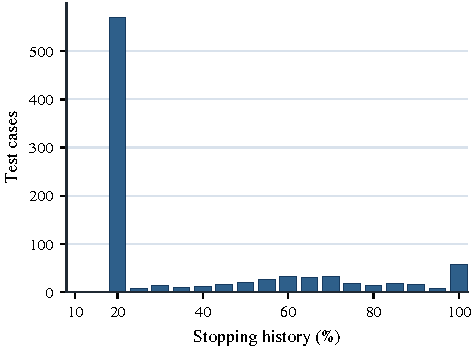
\includegraphics[width=\columnwidth]{figures/adaptive_stop_distribution.pdf}
    \caption{Held-out stopping-horizon distribution for the training-selected adaptive policy ($\tau=0.95$, $K=3$).}
    \label{fig:stopdist}
\end{figure}

\begin{table}[t]
\caption{Class-wise performance and stopping demand under the adaptive policy.}
\label{tab:adaptiveclass}
\centering
\scriptsize
\setlength{\tabcolsep}{3pt}
\begin{tabular}{lccc}
\toprule
Class & F1 & Mean stop (\%) & Stop $<100$ (\%) \\
\midrule
Normal & 0.9814 & 30.9 & 96.2 \\
Partial discharge & 0.8800 & 48.3 & 92.1 \\
Low-energy discharge & 0.8571 & 75.9 & 81.6 \\
Low-temp. overheating & 0.8276 & 71.4 & 78.0 \\
\bottomrule
\end{tabular}
\end{table}

The class-wise behavior in Table~\ref{tab:adaptiveclass} is operationally meaningful. Normal cases usually accumulate sufficient evidence quickly. Partial discharge requires more history, while low-energy discharge and overheating often require substantially longer observation. A fixed 75\% horizon therefore hides a real case- and class-dependent evidence requirement.

\subsection{Selective Diagnosis, Conformal Sets, and Horizon-Specific Explanation}
The original fixed-horizon selective analysis remains useful as a baseline. At 75\% history and native-score threshold $\tau=0.80$, the canonical temporal model accepts 854 of 900 cases (94.89\% coverage), reaches 97.78\% accepted-case accuracy and 0.9379 accepted-case macro-F1, and defers 46 cases. All four true classes remain represented among the accepted cases.

The conformal extension provides a complementary uncertainty view. At 75\% history and nominal 90\% target coverage, marginal empirical coverage is 90.56\%, mean prediction-set size is 1.014, and 94.89\% of test cases receive singleton sets. Class-conditional empirical coverages are 89.60\% for normal mode, 89.47\% for partial discharge, 95.92\% for low-energy discharge, and 96.34\% for overheating. These values are encouraging, but the minority calibration counts are small; they do not justify a claim of precise class-wise coverage in a different deployment population.

SHAP is also evaluated at the decision horizons rather than only at the endpoint \cite{lundberg2017shap}. Individual feature rankings change materially with available history: Spearman rank correlation is 0.620 between 50\% and 75\%, 0.529 between 75\% and 100\%, and 0.460 between 50\% and 100\%. The top-10 Jaccard overlap between 75\% and 100\% is only 0.25. Figure~\ref{fig:shapfamily} shows that broader feature-family attribution is more stable than individual ranks: statistical summaries remain the largest family, endpoint/change information is particularly prominent at 75\%, and local-dynamics share increases toward the endpoint.

\begin{figure}[t]
    \centering
    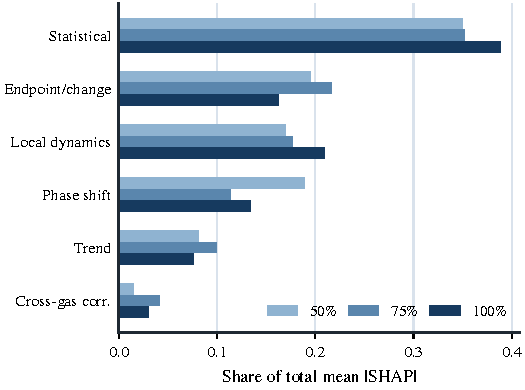
\includegraphics[width=\columnwidth]{figures/shap_family_by_horizon.pdf}
    \caption{Share of total mean absolute SHAP attribution by feature family at 50\%, 75\%, and 100\% history. Endpoint explanations should not be assumed to explain earlier decisions.}
    \label{fig:shapfamily}
\end{figure}

\subsection{Redundancy-Aware Feature Analysis}
The refinement experiment clarifies why the temporal representation works. Temporal-82 contains 82 nominal columns but only rank 70 after scaling; Temporal-70 removes exact dependencies and has rank 70. Under the convergence-stable training-only configuration, Statistical-28 reaches mean five-fold CV macro-F1 0.8249 at 75\%, Temporal-70 reaches 0.8617, and Temporal-82 reaches 0.8634. The full representation is therefore not gaining twelve independent dimensions from its nominal size.

More importantly, the strongest single augmentation of Statistical-28 is not the local-roughness family. Adding only first and last gas levels yields 36 features and raises training-CV macro-F1 to 0.8749. Its held-out test macro-F1 is 0.8907 versus 0.8946 for Temporal-82 under the same refinement configuration. The paired test difference is small relative to its uncertainty, so the evidence does not support a claim that the entire 82-column representation is necessary at 75\% history.

\begin{table*}[t]
\caption{Redundancy-aware 75\%-history ablation under the convergence-stable refinement configuration. Selection/interpretation should prioritize training-CV patterns; test values are held-out confirmation.}
\label{tab:ablationnew}
\centering
\footnotesize
\begin{tabular}{lcccc}
\toprule
Representation & Features & Rank & Training-CV macro-F1 & Test macro-F1 \\
\midrule
Statistical-28 & 28 & 28 & 0.8249 & 0.8390 \\
Stat28 + endpoint levels & 36 & 36 & \textbf{0.8749} & 0.8907 \\
Stat28 + local roughness & 40 & 40 & 0.8552 & 0.8734 \\
Temporal-70 nonredundant & 70 & 70 & 0.8617 & 0.8907 \\
Temporal-82 original & 82 & 70 & 0.8634 & 0.8946 \\
Temporal-70 minus trend & 62 & 62 & 0.8710 & 0.8820 \\
Temporal-70 minus correlations & 64 & 64 & 0.8677 & \textbf{0.8950} \\
\bottomrule
\end{tabular}
\end{table*}

The mechanism is therefore more precise than ``temporal dynamics compensate for incomplete history.'' Temporal anchoring---especially where the trajectory starts and where it currently stands---carries substantial incremental value. Local roughness also helps, while trend and cross-gas correlation features do not consistently improve training-CV performance. More temporal features are not automatically better.

\subsection{Robustness: Missingness Is Benign, High-Frequency Noise Is Not}
Under the advanced stress protocol, the clean 75\%-history Temporal-82 reference is 0.8971 macro-F1. Randomly removing 5\%, 10\%, or 20\% of timestamps and linearly interpolating them produces no observed prediction change in this benchmark. A single contiguous 20\% gap also remains close to the clean reference at 0.8958 mean macro-F1. These results should be interpreted narrowly: they show tolerance to the tested reconstruction process on these smooth trajectories, not universal immunity to missing data.

Gradual multiplicative drift is more damaging. Mean macro-F1 is 0.8956 at 5\% drift, 0.8794 at 10\%, and 0.8372 at 20\%. The strongest failure appears under independent high-frequency multiplicative Gaussian perturbation: Temporal-82 falls to 0.3179 mean macro-F1 at 2\% noise in the fixed-$C=30$ stress study. In the later convergence-stable refinement, the corresponding Temporal-82 value is even lower at 0.2476. This is a genuine negative result and should not be hidden behind the clean benchmark.

The refinement experiment tests a specific mitigation rather than searching a broad model zoo. Removing algebraic redundancy raises the 2\%-noise result from 0.2476 to 0.4292. A training-only OOF search over causal moving-average windows then selects $w=11$ among the predeclared candidates $\{1,3,5,7,11\}$ while satisfying the 98\% clean-retention constraint. On clean test data, the robust Temporal-70 model reaches 0.8964 macro-F1, compared with 0.8946 for the refinement Temporal-82; the paired difference is $+0.0018$ with 95\% CI $[-0.0195,0.0244]$. The appropriate conclusion is preservation of clean performance, not superiority.

Under independent test noise, the benefit is large but incomplete. At 2\% noise, robust Temporal-70 reaches 0.6250 versus 0.4292 for unsmoothed Temporal-70 and 0.2476 for Temporal-82. At 5\%, the corresponding values are 0.4691, 0.3989, and 0.2149. At 10\%, they are 0.4199, 0.3842, and 0.2048. Figure~\ref{fig:robust} includes the clean operating point to make the residual degradation explicit.

\begin{figure}[t]
    \centering
    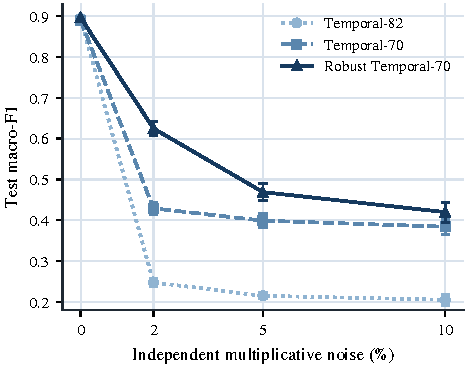
\includegraphics[width=\columnwidth]{figures/robustness_refinement.pdf}
    \caption{Clean and noise-stressed held-out macro-F1 in the final refinement. Causal smoothing and redundancy removal substantially mitigate the tested perturbation, but do not restore clean performance. Error bars show one standard deviation across 20 noise realizations.}
    \label{fig:robust}
\end{figure}

\section{Discussion and Engineering Implications}
\subsection{Observation Duration and Representation Are Coupled}
The strongest result is not the endpoint accuracy. High endpoint scores are already common in DGA machine-learning studies \cite{katser2022,hechifa2024ensemble,lv2024lightgbm,bouzar2026robustness}. The stronger result is that the relative value of a representation changes with the observation horizon. The formal interaction interval is entirely positive, and the dense curve shows where that interaction occurs: temporal information is most valuable in an intermediate partial-history regime, not uniformly from the first sample to the endpoint.

This resolves an apparent contradiction in the canonical results. At 100\%, Statistical-28 has the higher point estimate. At 75\%, Temporal-82 has the clear advantage. At 25\%, Statistical-28 is again better. The correct engineering interpretation is therefore not that ``temporal features are always better for incomplete history.'' It is that selected temporal anchoring and change descriptors carry additional information once enough trajectory has accumulated to estimate them reliably, but before the full distributional record has made them redundant.

\subsection{Adaptive Stopping Is More Useful Than a Universal 75\% Rule}
The fixed 75\% result remains valuable because it demonstrates that the temporal model can approach its own endpoint score with 105 fewer measurements. However, the adaptive experiment shows that a single global horizon is unnecessarily rigid. Easy cases, especially normal operation, often satisfy the persistent-evidence rule very early. Difficult low-energy-discharge and overheating cases frequently require more history. The resulting mean stopping horizon of 37.8\% is therefore not achieved by lowering a global cutoff; it emerges from case-specific evidence accumulation.

This suggests a practical stop/continue/defer architecture. A monitoring system should recompute the representation as new DGA measurements arrive, stop when persistent evidence is sufficient, continue when it is not, and defer unresolved endpoint cases for expert interpretation. Such a workflow converts confidence from a post-hoc score into an explicit observation-management policy.

\subsection{Compact Representations Can Be Stronger Engineering Choices}
The redundancy audit changes the explanation of why partial-history diagnosis works. The nominal 82-feature representation contains only 70 independent directions, and a 36-feature Statistical-28-plus-endpoint representation captures most of the 75\%-history benefit. This result argues against equating engineering sophistication with feature count.

The practical message is that temporal anchoring is more important than indiscriminate temporal complexity. First/current gas levels encode where the trajectory began and where it has arrived; local roughness adds complementary evidence; some trend and correlation descriptors are unnecessary or even counterproductive under training CV. This is favorable for deployment because smaller representations reduce computation, simplify auditability, and can reduce perturbation amplification.

\subsection{Robustness Must Be Demonstrated, Not Assumed}
The stress tests expose a mixed robustness profile. Interpolated missing timestamps and contiguous gaps are surprisingly benign on this benchmark. Drift produces a gradual and interpretable decline. High-frequency independent multiplicative noise, however, causes catastrophic degradation in the original temporal representation. The failure is consistent with the design of first-difference and maximum-step descriptors: perturbations that are small relative to absolute gas level can dominate local-difference statistics when the underlying trajectories are smooth.

The mitigation experiment is deliberately narrow. Redundancy removal improves stability, and causal smoothing improves it further while preserving clean performance. Even so, 2\%-noise macro-F1 remains 0.6250, far below the clean 0.8964. The correct claim is therefore \emph{material mitigation}, not complete noise robustness. This negative result strengthens the engineering credibility of the study because it identifies a condition under which the clean benchmark is not reliable.

\subsection{Explanation and Uncertainty Must Match the Decision Horizon}
The SHAP stability results show that endpoint explanations should not be reused as if they explained earlier decisions. Individual ranking correlations between horizons are only moderate and the 75/100 top-10 overlap is 0.25. Broader family and gas-level patterns are more stable, so engineering interpretation should emphasize groups of correlated descriptors rather than overinterpreting one coefficient or SHAP rank.

Likewise, score-based abstention and conformal sets serve different purposes. Native scores provide a convenient ranking signal for adaptive stopping. Split conformal prediction gives a fixed-horizon uncertainty set with an explicit nominal coverage target under its assumptions. Neither eliminates the need for engineering judgment, and the sequential use of ordinary split-conformal sets should not be described as an anytime-valid guarantee.

\subsection{Role in Maintenance Decision Support}
The proposed system should be treated as decision support, not an autonomous protection or maintenance controller. A practical interface can show the recent DGA trajectories, predicted class, observation horizon, dominant feature families, uncertainty or accept/defer status, and the reason a case has stopped or remained under monitoring. A persistent high-confidence discharge or overheating prediction can prompt engineering inspection, while a boundary case can remain under observation or be escalated for expert interpretation.

This human-in-the-loop design aligns with the role of engineering judgment in established DGA guidance \cite{ieeeC57104,iec60599}. It also avoids the misleading implication that a benchmark classifier alone should determine transformer switching, protection, or replacement actions.

\section{Related Work}
\subsection{Conventional DGA Interpretation}
DGA has a long history in transformer condition assessment. Rogers formalized gas-ratio interpretation for incipient faults in 1978 \cite{rogers1978}, and modern IEEE and IEC guidance incorporates gas-generation theory, concentrations, ratios, trends, and case-specific interpretation \cite{ieeeC57104,iec60599}. Reviews by Cheng and Yu \cite{cheng2018survey}, Ali \emph{et al.} \cite{ali2023review}, and Nanfak \emph{et al.} \cite{nanfak2024review} document the evolution from deterministic ratio and graphical methods toward hybrid and intelligent approaches. These methods establish the engineering context for data-driven diagnosis, but several conventional ratio techniques require gases that are absent from the four-channel benchmark used here.

\subsection{Machine Learning for Transformer Fault Diagnosis}
A wide range of machine-learning methods have been applied to DGA. Zhang \emph{et al.} combined feature selection with an optimized SVM \cite{zhang2019khsvm}; Shang \emph{et al.} coupled a multiclass SVM with Dempster--Shafer evidence fusion \cite{shang2019hmsvm}; Liu \emph{et al.} used correlation-based DBSCAN clustering \cite{liu2020dbscan}; and Hechifa \emph{et al.} compared multiple DGA feature vectors with tree ensembles \cite{hechifa2024ensemble}. Lv \emph{et al.} proposed a dual-branch LightGBM ensemble and explicitly addressed imbalance and feature representation \cite{lv2024lightgbm}. Zhang \emph{et al.} modeled dependence among gases using a copula-based representation \cite{zhang2022copula}. The breadth of this literature makes another endpoint classifier comparison a weak research contribution by itself.

\subsection{Temporal DGA, Robustness, and the Gap Addressed Here}
Temporal DGA work often focuses on future gas prediction or health-state forecasting. Qi \emph{et al.} developed a deep recurrent belief network for DGA trend prediction and emphasized temporal correlation in online monitoring \cite{qi2019drbn}. In the benchmark lineage used here, Katser \emph{et al.} used automated time-series feature extraction and classical models on complete histories \cite{katser2022,christ2018tsfresh}. Their work shows that strong endpoint diagnosis is possible without relying exclusively on deep networks.

Recent review work emphasizes a broader accuracy--robustness gap in AI-based DGA, including measurement uncertainty, validation practices, distribution shift, and interpretability \cite{bouzar2026robustness}. The present study addresses one concrete part of that gap. We treat the amount of observed history as an independent variable, formally test the horizon--representation interaction, select an adaptive stopping policy without test-set tuning, quantify fixed-horizon uncertainty, and expose performance under controlled missingness, drift, and noise. The contribution is therefore not a new classifier family; it is a validated observation-management and representation-design framework for lightweight DGA diagnosis.

\section{Limitations and Threats to Validity}
The findings are strong within the benchmark but should not be generalized beyond the evidence. First, the study uses one public dataset and one predefined test split. We have not established that the intermediate-horizon interaction, adaptive stopping distribution, or robust smoothing choice transfers to another transformer fleet, oil chemistry, sensor platform, or utility. External validation remains the most important next step.

Second, the benchmark contains only H$_2$, CO, C$_2$H$_4$, and C$_2$H$_2$. It does not contain the full gas set required by several established DGA methods. A direct comparison with every Rogers, IEC-ratio, Duval-triangle, or pentagon formulation would therefore be incomplete or unfair.

Third, the minority classes remain small: the held-out set contains only 38 partial-discharge and 49 low-energy-discharge cases. Macro-F1, balanced accuracy, paired resampling, class-specific stopping statistics, and conformal coverage expose this limitation but cannot create information that the dataset does not contain. The class-conditional conformal calibration subsets are correspondingly small, so their class-wise coverage estimates are imprecise.

Fourth, truncating complete histories is a retrospective simulation of earlier diagnosis. It prevents future-feature leakage but does not establish prospective fault onset or prove that a maintenance action could have been taken the corresponding number of days earlier. The adaptive stopping policy therefore estimates how much of this benchmark history is sufficient for classification, not the clinical or physical lead time to fault occurrence.

Fifth, the robustness tests are controlled synthetic stress tests. Linear interpolation may be unusually effective because the benchmark trajectories are smooth. Likewise, independently injected multiplicative Gaussian perturbation is intentionally demanding and is not claimed to be a calibrated field sensor-error model. The selected $w=11$ causal smoothing window is the best among the predeclared candidate set, not a universally optimal filter.

Finally, the canonical and extension/refinement experiments use deliberately separated numerical protocols. Canonical values remain tied to the original $C=30$, unweighted paper archive. Dense/adaptive analyses use the same fixed classifier with a tighter solver tolerance, while the final redundancy/noise study reselects the convergence-stable configuration using training CV only. This separation prevents test-set-driven retrofitting but means that small score differences across sections should not be interpreted as repeated measurements of one identical fitted model.

\section{Conclusion}
This paper changes the usual DGA machine-learning question from ``which classifier reaches the highest endpoint score?'' to ``how should observation duration, representation, uncertainty, and stopping be designed so that a reliable diagnosis is issued as soon as sufficient evidence is available?'' Using leakage-safe prefixes from 3,000 transformer histories and training-only selection, the experiments show that the answer is inherently horizon dependent.

The canonical Temporal-82 model reaches 0.8971 macro-F1 at 75\% history and 0.9026 at 100\%, retaining 99.39\% of endpoint performance. More importantly, the formal paired interaction is 0.0761 with 95\% CI $[0.0278,0.1263]$, confirming that temporal representation has greater incremental value at 75\% than at the endpoint. Dense evaluation further shows that this advantage is concentrated mainly in an intermediate partial-history regime rather than being universal.

A training-selected adaptive policy then removes the need to force every case to the same horizon. With $\tau=0.95$ and persistence $K=3$, it obtains 0.8865 test macro-F1, retains 98.29\% of its endpoint reference, and stops at 37.8\% history on average; 93.6\% of cases stop before 100\%. Fixed-horizon class-conditional conformal prediction provides approximately the requested 90\% coverage at 75\%, while horizon-specific SHAP shows that explanations themselves change as evidence accumulates.

The refinement results also narrow the mechanism. Temporal-82 has numerical rank 70, a compact 36-feature statistical-plus-endpoint representation captures much of the 75\%-history benefit, and some trend/correlation descriptors add little under training CV. Controlled robustness tests reveal a severe high-frequency-noise failure that is substantially mitigated by redundancy removal and causal smoothing: at 2\% synthetic multiplicative noise, macro-F1 improves from 0.2476 for Temporal-82 to 0.6250 for the robust Temporal-70 representation while clean performance remains near 0.896. The improvement is large, but the residual degradation is real.

The resulting engineering message is direct. A practical lightweight DGA system should not wait blindly for a fixed endpoint, should not assume that one feature representation is best at every horizon, and should not treat clean benchmark accuracy as evidence of robustness. It should stop when persistent evidence is sufficient, continue when it is not, expose uncertainty and explanations at the actual decision horizon, and defer unresolved cases to engineering judgment.

\section*{Data and Reproducibility}
The Power Transformers FDD and RUL dataset is publicly available under CC0 and provides the original 2,100 training and 900 test cases used here \cite{katserDataset}. All shorter-horizon features are computed from prefixes before feature extraction. The package accompanying this manuscript preserves three evidence layers: the canonical five-fold paper outputs, the convergence-stabilized advanced dense/adaptive/conformal/SHAP/robustness outputs, and the final redundancy/noise refinement outputs. Paired comparisons archive exact per-case predictions where required, and the refinement archive records environment information and feature-extractor validation to numerical precision. These artifacts are included with the LaTeX source so that every reported extension can be traced to a machine-readable result file.

\balance
\bibliographystyle{IEEEtran}
\bibliography{references}

\end{document}
